\documentclass[10pt]{beamer}
\usetheme[
%%% option passed to the outer theme
%    progressstyle=fixedCircCnt,   % fixedCircCnt, movingCircCnt (moving is deault)
  ]{Feather}
  
% If you want to change the colors of the various elements in the theme, edit and uncomment the following lines

% Change the bar colors:
%\setbeamercolor{Feather}{fg=red!20,bg=red}

% Change the color of the structural elements:
%\setbeamercolor{structure}{fg=red}

% Change the frame title text color:
%\setbeamercolor{frametitle}{fg=blue}

% Change the normal text color background:
%\setbeamercolor{normal text}{fg=black,bg=gray!10}

%-------------------------------------------------------
% INCLUDE PACKAGES
%-------------------------------------------------------

\usepackage[utf8]{inputenc}
\usepackage[english]{babel}
\usepackage[T1]{fontenc}
\usepackage{helvet}
\usepackage{multirow}

%-------------------------------------------------------
% DEFFINING AND REDEFINING COMMANDS
%-------------------------------------------------------

% colored hyperlinks
\newcommand{\chref}[2]{
  \href{#1}{{\usebeamercolor[bg]{Feather}#2}}
}

%-------------------------------------------------------
% INFORMATION IN THE TITLE PAGE
%-------------------------------------------------------

\title[] % [] is optional - is placed on the bottom of the sidebar on every slide
{ % is placed on the title page
      \textbf{Complete The Look Recommendation with Street Fashion Images}
}

\subtitle[Complete The Look Recommendation]
{
%      \textbf{v. 1.0.0}
}

\author[Bhaskar Bagchi]
{      Bhaskar Bagchi \\
      {\ttfamily bagchi.bhaskar@cse.iitkgp.ernet.in}
}

\institute[]
{
      Department of Computer Science and Engineering\\
      Indian Institute of Technology, Kharagpur\\
  
  %there must be an empty line above this line - otherwise some unwanted space is added between the university and the country (I do not know why;( )
}

\date{\today}

%-------------------------------------------------------
% THE BODY OF THE PRESENTATION
%-------------------------------------------------------

\begin{document}

%-------------------------------------------------------
% THE TITLEPAGE
%-------------------------------------------------------

{\1% % this is the name of the PDF file for the background
\begin{frame}[plain,noframenumbering] % the plain option removes the header from the title page, noframenumbering removes the numbering of this frame only
  \titlepage % call the title page information from above
\end{frame}}


\begin{frame}{Content}{}
\tableofcontents
\end{frame}

%-------------------------------------------------------
\section{Introduction}
%-------------------------------------------------------
\subsection{Problem Definition}
\begin{frame}{Introduction}{Problem Definition}
%-------------------------------------------------------

  \begin{itemize}
    \item<1-> Given an item(clothing) in the shopping cart the problem statement is to suggest items complementary to it which may contain garments or accessories which makes a complete set as per current fashion.
%    \item<2-> The rest of the theme is provided under the GNU General Public License v. 3 (GPLv3) \chref{http://www.gnu.org/licenses/}{http://www.gnu.org/licenses/}. This means that you can redistribute it and/or modify it under the same license. 
  \end{itemize}
\end{frame}


\begin{frame}{Introduction}{Problem Definition}
\begin{figure}[t]
    \centering
    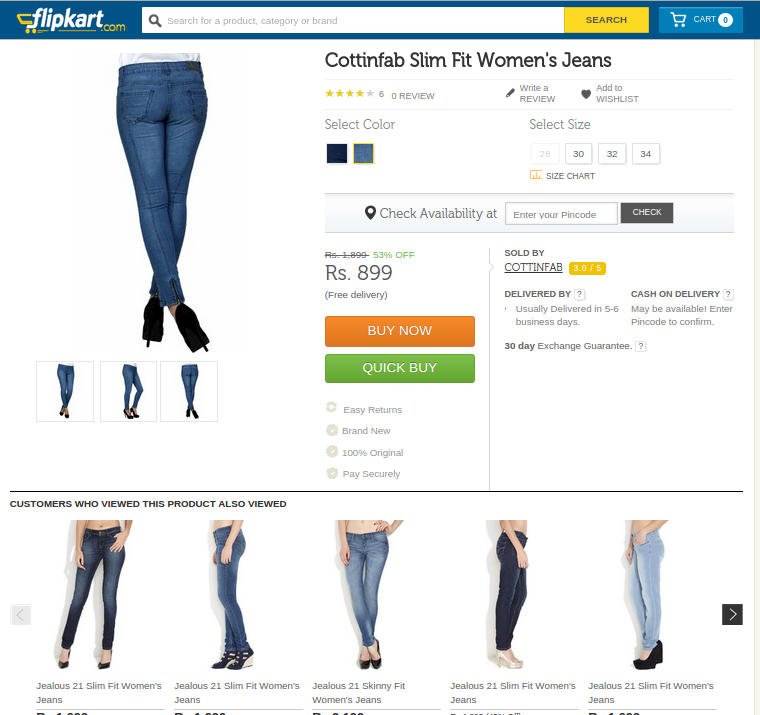
\includegraphics[height=\dimexpr11\textheight/16\relax]{reco_exst_1}
    \caption{Existing Recommendation Systems}
  \end{figure}
\end{frame}



\begin{frame}{Introduction}{Problem Definition}
\begin{figure}[t]
    \centering
    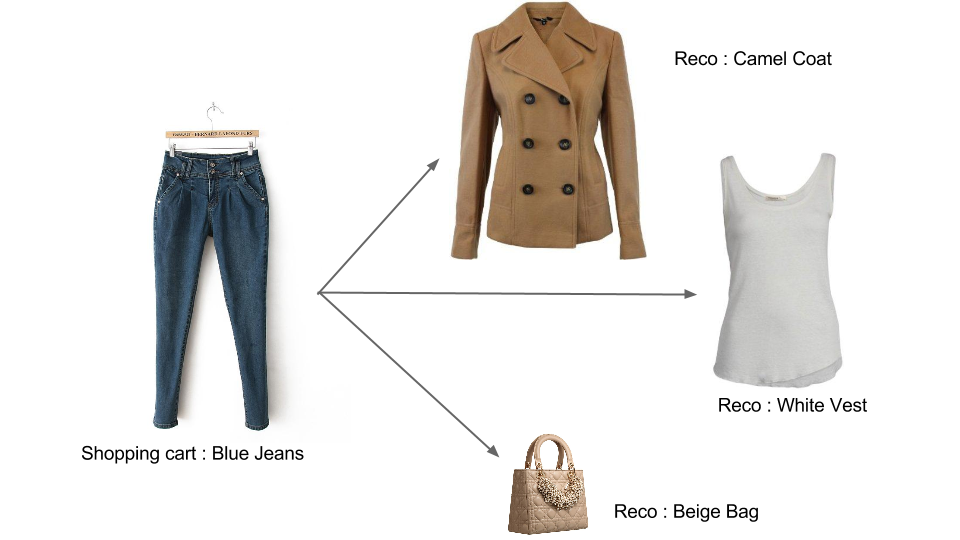
\includegraphics[height=\dimexpr11\textheight/16\relax]{Untitled}
    \caption{Visualization of the problem statement}
  \end{figure}
\end{frame}


%-------------------------------------------------------
\section{Mathematical Formulation}
%-------------------------------------------------------
\subsection{Feature Representation}
% \begin{frame}{Mathematical Formulation}{Feature Representation}
% %-------------------------------------------------------

% \begin{itemize}
%   \pause
%   \item<1-> Say we have n training images.
%   \pause
%   \item<2-> Each image `\emph{i}' has `\emph{p}' parts.
%   \pause
%   \item<3-> Each part is represented by a \emph{k-dimensional} feature vector, \emph{h}.
% \end{itemize}

% \pause

% \begin{block}{}
% Thus each can be represented as follows:
% \begin{itemize}
% \item {\tt Image H$_{i}${$^{T}$} = [h$_{i1}${$^{T}$}, h$_{i2}${$^{T}$},... , h$_{ip}${$^{T}$}].}
% \item {\tt Dataset H = [H$_{1}$, H$_{2}$,... , H$_{n}$]}
% \end{itemize}
% \end{block}

% \pause
% \begin{block}{}
% The recommendation task will be to generate a predictive model \emph{M}(\emph{H},\emph{q}), where \emph{H} is the training set and given some query \emph{q} with some part m missing, we can predict the m$^{th}$ part.
% \end{block}

% \end{frame}


% %-------------------------------------------------------
% \subsection{Simplified Formulation}
% \begin{frame}{Mathematical Formulation}{Simplified Formulation}
% %-------------------------------------------------------
%   The previous formulation is very rigid, where each image has to have \emph{p} parts. So we have following relaxation.
%   \pause
%   \begin{block}{Relaxations}
%   \begin{itemize}    
%     \item Instead of asserting each image to have \emph{p} parts we keep it flexible.
%     \item We also don't define any particular order of parts of clothings.
%     \item Instead of using numeric features we use textual tags corresponding to each part of the garment/accessory as feature.
%     \item Thus each image is defined by a number of features, which are 2--tuples $\{ Cloth-type \: {:} \: Cloth-description/color \}$.
%   \end{itemize}
%   \end{block}
% \end{frame}

\begin{frame}{Mathematical Formulation}{Simplified Formulation}
\begin{block}{}
Given an image $i$ containing `$k$' part--features, we describe the image $P_i$ as $P_i^{T} := [p_{i1}, p_{i2}, ..., p_{ik}]$ where each $p_{ij}$ are textual part--features, which are 2--tuples.
\end{block}
\pause
\begin{block}{}
We learn a model from our dataset of fashion images, say \textbf{P}, where \textbf{P} := $[P_1, P_2, ... P_n]^{T}$.
\end{block}
\pause
\begin{block}{}
The task of our recommendation system is, given one or more apparel, and corresponding part features $p$'s as input query, recommend garments which can be worn with it/them as a set.
\end{block}
\end{frame}     

%-------------------------------------------------------
% \section{Approach}
% \subsection{Basic Approach}
% \begin{frame}{Approach}{Basic Approach}
% %-------------------------------------------------------

% \begin{enumerate}
% 	\pause
% 	\item Make a bipartite graph where one of the partite sets is \emph{images} and the other is  \emph{features}. Edge exists if feature is present in the image.
%     \pause
%     \item Take the projection of this graph on the feature set, thus we get the co--occurrence graph.
%     \pause
%     \item For given query part--feature, calculate its SimRank with its neighbours and return the k--nearest--neighbours.
%     \pause
%     \item In case of more than one feature--parts in the query, for each part find the k--nearest--neighbours.
%     \pause
%     \item For each k--nearest--neighbour list combine them into a single list using \emph{Broda's Rank Aggregation}.
% \end{enumerate}
% \end{frame}

\begin{frame}{Approach}{Flow Diagram}
\begin{figure}[t]
    \centering
    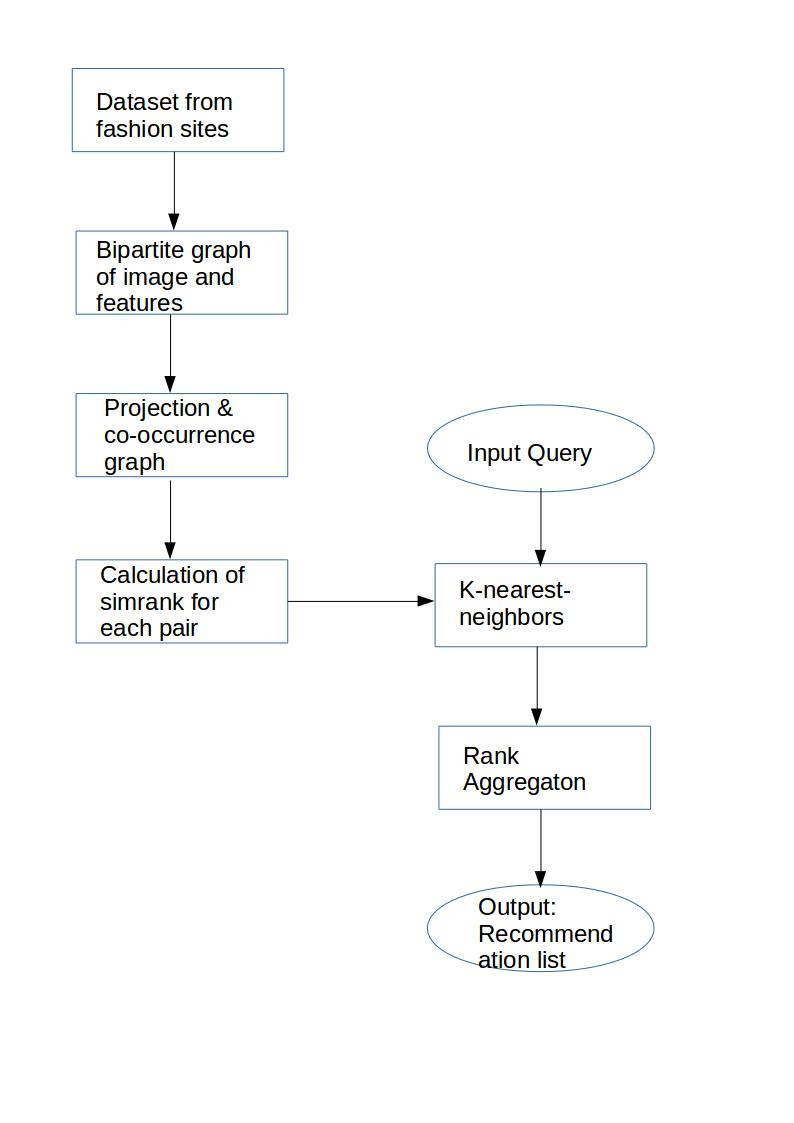
\includegraphics[height=\dimexpr11\textheight/16\relax]{flowchart}
    \caption{Flow Diagram of Proposed Approach}
  \end{figure}
\end{frame}

\subsection{Fashion Websites \& Ground Truth}
\begin{frame}{Fashion Websites \& Ground Truth}{Scraping Fashion Websites}
\begin{itemize}
\item Scraped more than 500 images of female fashionstas from \url{www.chictopia.com}. These images covered an appreciable range of street fashion from corporate dressing sense to the most casual of the dresses.
\pause
\item Created a vocabulary of part features. Manually normalize the tags associated with each image.
\pause
\item Ended up with a codebook of total of \textit{48} unique categories including garments like tops, jeans, etc. and accessories like watches, bracelets, etc. and \textit{632} unique items i.e. category-description pair.
\end{itemize}
	%\begin{figure}[t]
    %\centering
    %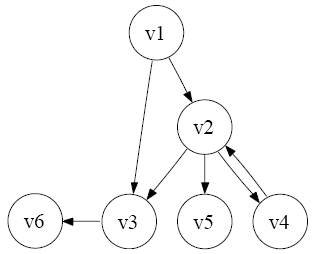
\includegraphics[scale=0.3]{simrank}
    %\caption{Directed graph representing websites and hyperlinks}
  	%\end{figure}
\end{frame}


\subsection{Bipartite Network and Co--occurrence Graph}
\begin{frame}{Bipartite Network and Co--occurrence Graph}{}
\begin{itemize}
\item A bipartite graph is formed with dataset images $P$'s as the first partite sets and part--features $p_i$'s as the second partite set. There exists an edge between ever part feature and the image in which it occurred.
\pause
\item The bipartite graph is then projected to the set of part features.
\pause
\item The projected graph so obtained is a weighted co--occurrence graph of the part features. Construction of this graph gives us the relation between different garments and accessories which can be used together and are complementary to each other.
\pause
\item This step helps us learn a correlation and inter-dependence between various part features from the dataset.
\end{itemize}


%Mathematically SimRank score is defined recursively. Let us denote similarity between objects a and b by S(a, b) $\in$ [0, 1].
%\begin{block}{Formula}
%\begin{equation}
%S(a, b) =	\left\{ \begin{array}{ll}
%			1 & \mbox{if $a=b$}; \\
%			\frac{C}{\left | I(a) \right | \left | I(b) \right |}\sum_{i = 0}^{\left | I(a) \right |}\sum_{j = 0}^{\left | I(b) \right |}S\left(I_i\left(a\right), I_j\left(b\right ) \right) & \mbox{$otherwise$}.\end{array} \right.
%\end{equation}

%where, \emph{C} is a constant between 0 and 1 which controls the amount of score propagation in recursive call, \emph{I(a)} is the set of incoming edges to a and \emph{I(b)} is the set of incoming edges to b.

%\end{block}
\end{frame}

\subsection{Similarity Measure \& Nearest Neighbor Consensus}
\begin{frame}{Similarity Measure \& Nearest Neighbor}{Similarity Measure}
\begin{itemize}
\item The co-occurrence graph falls in a domain where nodes represents the objects and edges represents the relations between them. We use \textit{Simrank} to measure the similarity based on \textit{structural context} of the graph.
\pause
\item Convert the co--occurrence graph into a directed graph where each edge between part features $p_a$ and $p_b$ in the original graph is replaced by two directed edges $p_a \rightarrow p_b$ and $p_b \rightarrow p_a$ both with weights equal to the weight of original edge.
\pause
\item Compute \textit{Simrank} between each pair of nodes.
\end{itemize}

%\pause
%\begin{block}{Types of rank aggregation problems}
%\begin{enumerate}
%\item If the individual lists contain all the elements in \emph{U} then they are called complete lists. They are a total ordering of \emph{U}.
%\item There are situations where full lists are not convenient, and even not possible. In such cases the lists contain an ordered list of a subset of elements of \emph{U}. $ \left | L_i \right | < \left | U \right |$. Such lists are called partial lists.
%\item A special case of the partial list problem is the top--K list. In this ranking we take the top K elements from each ordered list, and so we know that all the elements that are not present in the list are ranked below those which are present in the list.
%\end{enumerate}
%\end{block}
\end{frame}

\begin{frame}{Similarity Measure \& Nearest Neighbor}{Nearest Neighbor Consensus}
\begin{itemize}
\item Given a part--feature $p$ as query we locate the node corresponding to that part feature in the co--occurrence graph.
\pause
\item We find out other nodes which are close to it, i.e. nodes which have highest simrank value with this node.
\pause
\item The rationale behind this step is that since the graph had edges between part features that were used together by fashionistas and as the simrank values decrease with increase in node distances, the $k$--nearest--neighbors will be those part features which were frequently used with the selected item and are contemporary to it.
\pause
\item We get a list of k part features $p_1, p_2, ... p_k$ which are structurally close to the input feature and thus they can be recommended for the given query part feature.
\end{itemize}
\end{frame}

\subsection{Aggregating Ranked Item Recommendations}
\begin{frame}{Aggregating Ranked Item Recommendations}{Rank Aggregation}
\begin{itemize}
\item Say we have $j$ part features $p_1, p_2, ... p_j$ as input query, we find out individual $k$--nearest--neighbors for each part feature.
\pause
\item we have $j$ ranked lists, each with $k$ members, which are recommendation related to each input feature.
\pause
\item Assigns a score corresponding to position in which a part feature appears within each ranked list. In our case, for each list $i$, ${p_a}^i$ is assigned a weight ${B_{p_a}}^i$ = $k$ * fraction of part features in the list appearing below $p_a$.
\pause
\item The \textit{Broda} score of each element $B_{p_a}$ is the the sum of \textit{Broda} scores for that part feature in all the lists.
\pause
\item We can recomment the top $k$ elements from this ranked list to the user.
\end{itemize}
\end{frame}


%-------------------------------------------------------
\section{Experimental Results}
\begin{frame}{Experimental Results}{Evaluation Methodology}
%-------------------------------------------------------
\begin{itemize}
\item We took 20 images as test set from our dataset. Since each image is user tagged, we have labelled ground truth for computing the required metrics.
\pause
\item For each image we took, we used all its part features individually as one feature input. We also used various permutations of 2 part features and 3 part features as input to the recommender and compared the recommended part features with the ground truth.
\pause
\item Then we calculated \textit{precision, recall} and \textit{f1} values for 158 sets of recommendations.
\end{itemize}
\pause
\begin{block}{Formula}
$precision = \frac{no \ of \ matched \ recommendations}{no \ of \ recommendations}$
\newline
$recall = \frac{no \ of \ matched \ recommendation}{no \ of \ items \ in \ actual \ image}$
\end{block}
\end{frame}

\begin{frame}{Experimental Results}{Results}
Out of the 158 recommendation sets that we tested, 53 were 1 part feature input, 54 were 2 part feature input and 51 as 3 part feature input. For each generated recommendations we calculated the precision and recall.

\begin{table}
\centering
\caption{Precision}
\begin{tabular}{|c|c|c|c|}
\hline
No. of inputs & Max Precision & Avg Precision\\
\hline\hline
1 & 1 & 0.31\\
2 & 0.75 & 0.31\\
3 & 0.6 & 0.28\\
\hline\end{tabular}
\label{table:precision}
\end{table}

\begin{table}
\centering
\caption{Recall}
\begin{tabular}{|c|c|c|c|}
\hline
No. of inputs & Max Recall & Avg Recall\\
\hline\hline
1 & 0.8 & 0.23\\
2 & 1 & 0.44\\
3 & 1 & 0.48\\
\hline\end{tabular}
\label{table:recall}
\end{table}
\end{frame}

\begin{frame}{Experimental Results}{Results}
\begin{table}
\centering
\caption{f1 score}
\begin{tabular}{|c|c|c|}
\hline
No. of inputs & Max f1 & Min f1\\
\hline\hline
1 & 0.89 & 0.13\\
2 & 0.71 & 0.1\\
3 & 0.67 & 0.1\\
\hline\end{tabular}
\label{table:f1}
\end{table}
\begin{figure}[htb]
\centering
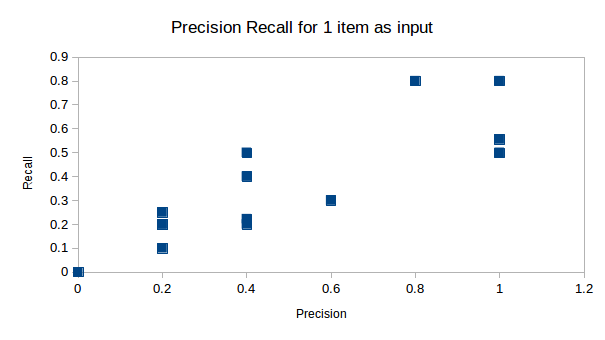
\includegraphics[scale=0.4]{g11}
\caption{Precision-Recall for 1 item input}
\label{fig:g1}
\end{figure}
\end{frame}

\begin{frame}{Experimental Results}{Precision Recall Graphs}
\begin{figure}[htb]
\centering
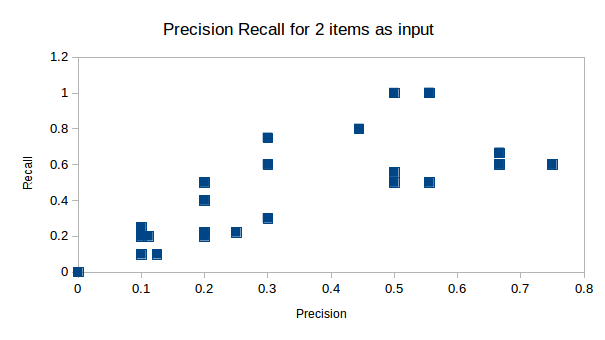
\includegraphics[scale=0.4]{g22}
%\caption{Precision-Recall for 2 item input}
\label{fig:g2}
\end{figure}
\begin{figure}[htb]
\centering
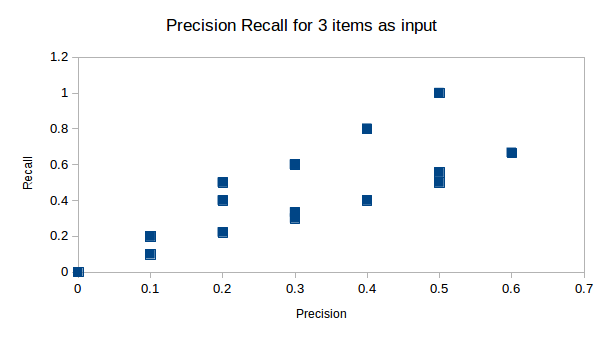
\includegraphics[scale=0.4]{g33}
%\caption{Precision-Recall for 3 item input}
\label{fig:g3}
\end{figure}
\end{frame}

\begin{frame}{Experimental Results}{Manual Evaluation Results}
\begin{table}
\centering
\caption{User rating for recommendation}
\begin{tabular}{|c|c|c|}
\hline
Rate(out of 10) & Frequency & Cumulative Freq.\\
\hline\hline
10 & 1 & 1\\
9 & 2 & 3\\
8 & 9 & 12\\
7 & 9 & 21\\
6 & 5 & 26\\
5 & 11 & 37\\
4 & 11 & 48\\
3 & 6 & 54\\
2 & 4 & 58\\
1 & 2 & 60\\
\hline\end{tabular}
\label{table:userRating}
\end{table}

\end{frame}

%-------------------------------------------------------
\section{Future Work}
\begin{frame}{Future Work}
%-------------------------------------------------------

\begin{itemize}

\item Features for representation of parts are to be improved by incorporating visual features. Inclusion of visual features will also include the analysis of features like color, texture, etc. which is expected to improve the quality of evaluation.

\item A feedback system can be added to the system as to increase edge weights to the features which are shopped together by users. This will be a self learning system and incorporate the changes in trending fashion all by itself.

\end{itemize}

\end{frame}

%-------------------------------------------------------
\section{References}
\begin{frame}{References}
%-------------------------------------------------------

\bibliographystyle{abbrv}
%\bibliography{sigproc}

\begin{thebibliography}{1}

\bibitem{rankAggregation}
C.~Dwork, R.~Kumar, M.~Naor, and D.~Sivakumar.
\newblock Rank aggregation methods for the web.
\newblock In {\em Proceedings of the 10th International Conference on World
  Wide Web}, WWW '01, pages 613--622, New York, NY, USA, 2001. ACM.

\bibitem{simrank}
G.~Jeh and J.~Widom.
\newblock Simrank: A measure of structural-context similarity.
\newblock In {\em Proceedings of the Eighth ACM SIGKDD International Conference
  on Knowledge Discovery and Data Mining}, KDD '02, pages 538--543, New York,
  NY, USA, 2002. ACM.

\bibitem{bundleReco}
T.~Zhu, P.~Harrington, J.~Li, and L.~Tang.
\newblock Bundle recommendation in ecommerce.
\newblock In {\em Proceedings of the 37th International ACM SIGIR Conference on
  Research \&\#38; Development in Information Retrieval}, SIGIR '14, pages
  657--666, New York, NY, USA, 2014. ACM.

\end{thebibliography}
\end{frame}


{\1
\begin{frame}[plain,noframenumbering]
  \finalpage{Thank you! Questions?}
\end{frame}}

\end{document}